\section{Challenges for imaging MeerKAT data} \label{meerkat}

There are several challenger for imaging meerkat data. One problem is the new amount of data.

terabytes of measurements. Large image size 32k squared are the obvious problems to solve. Distributing the problem is not part of this work.

 In this work, it is focused on Wide field of view issue. 


Calibration gets not explicitly called, but 

Further issues that do not get handled here
\begin{itemize}
	\item (Beam Pattern, A Projection)
	\item Full polarization
	\item Wide band imaging
\end{itemize}



\subsection{Wide Field of View Imaging} \label{wof}

So far the small Field of View inverse problem has been introduced where each antenna pair measures a Visibility of the sky brightness distribution. This leads to the small Field of View measurement equation \eqref{radio:eq:2dft}. It is identical to the two dimensional Fourier Transform. In practice the Fast Fourier Transform (FFT) is used, since it scales with $~n\:log(n)$ instead of $~n^2$ pixels.

\begin{equation}\label{radio:eq:2dft}
V(u, v) = \int\int x(l, m) e^{2 \pi i (ux+vy)} dl dm
\end{equation}

For wide Field of View imaging, two effects break the two dimensional Fourier Transform relationship: Non-coplanar Baselines and the celestial sphere which lead to the measurement equation \eqref{radio:eq:ftSphere}. Note that for small Field of View $1 - x^2 -y ^2 \ll 1$, and \eqref{radio:eq:ftSphere} reduces to the 2d measurement equation \eqref{radio:eq:2dft}.

\begin{equation}\label{meerkat:ftsphere}
	V(u, v, w) = \int\int \frac{X(x, y)}{\sqrt{1 - x^2 - y ^2}} e^{2 \pi i (ux+vy+ w\sqrt{1 - x^2 - y ^2})}dx dy
\end{equation}

\begin{wrapfigure}{r}{0.5\textwidth}
	\centering
	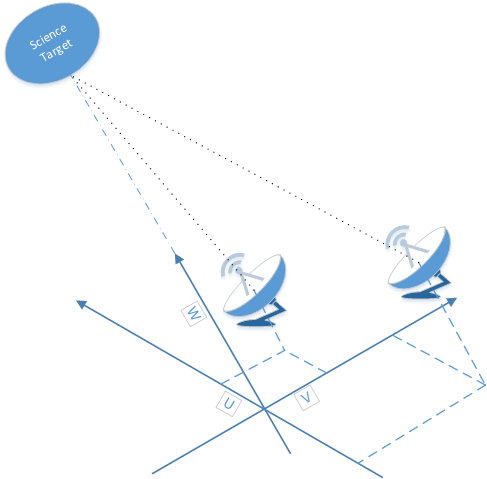
\includegraphics[width=0.9\linewidth]{./chapters/03.radio/uvw.png}
	\caption{U V and W coordinate space}
	\label{radio:uvw}
	\vspace{-10pt}
\end{wrapfigure}

Non-coplanar Baselines lead to a third component $w$ for each Visibility. Figure \ref{radio:uvw} shows the the $u$ $v$ and $w$ coordinate system. $w$ is essentially the pointing direction of the instrument. The UV-Plane is the projection of the antennas on a plane perpendicular to the pointing direction. Which point in the UV-Plane get sampled and what $w$ component it has depends on the pointing direction. If the instrument points straight up, the UV-Plane is a tangent to earth's surface, and the $w$ term compensates for earth's surface curvature. If however the instrument points at the horizon, the projected UV-Plane gets squashed and $w$ compensates for antennas which lie far behind the UV-Plane. In essence, $w$ is a phase delay that corrects antenna positions in three dimensions. The wide Field of View measurement equation \eqref{radio:eq:ftSphere} would account for the $w$ phase delay, but it breaks the the two dimensional Fourier relationship and the FFT cannot be used. The W-Projection \cite{cornwell2008noncoplanar} algorithm approximates the effect of the $w$ term restores the two dimensional Fourier relationship.


\subsection{State of the Art: Distributing the W-Term with WSCLEAN} 





Tackling the problem
State of the Art:Distributing the W-Term with WSCLEAN

Spherical Harmonics

FFT

uv smooth

Coordinate Descent



A-Projection \cite{bhatnagar2008correcting}







